\documentclass[
hidelinks,
12pt,
openany,
oneside,
a4paper,
chapter=TITLE,
portuguese, % ou english
]{abntex2}

\usepackage{config}
\makeglossaries
\begin{document}
\begin{OnehalfSpace}
\begin{center}
            \begin{figure}[htbp]
                \centering
                
\includegraphics[width=13cm]{assets/unologo-enhanced.png}
            \end{figure}
        
            \MakeUppercase{\textbf{Universidade Comunitária da Região de Chapecó}} \\
            \MakeUppercase{\textbf{ÁREA DE CIÊNCIAS EXATAS E AMBIENTAIS}}\\
            \MakeUppercase{\textbf{Ciência da Computação}}\\
            \MakeUppercase{\textbf{(BACHARELADO)}}\\
            
            \vspace{4.5cm}
            
            \MakeUppercase{\textbf{TÍTULO}}
            
            \vspace{3.5cm}
            
            \MakeUppercase{\textbf{ALUNO ALUNO ALUNO}}
            
            \vfill
            
            \MakeUppercase{\textbf{Chapecó, novembro DE 2024}} 
         
\end{center}
\clearpage

\pagenumbering{roman}
\textual
\pagestyle{simple} % tira cabeçalho com nome do capítulo e exibe só paginação
\setcounter{page}{2}
    \begin{center}
    \vspace{1cm}
    
    \textbf{\MakeTextUppercase{Universidade Comunitária da Região de Chapecó}\\}
    \textbf{\MakeTextUppercase{Área de ciências exatas e ambientais}\\}
    \textbf{\MakeTextUppercase{Ciência da Computação}\\}
    \textbf{\MakeTextUppercase{(Bacharelado)}\\}

    \vspace{6cm}

    % \MakeUppercase{\textbf{Protótipo de plataforma de dados escalável para processamento Big Data, utilizando dados  da agricultura}}
    \MakeUppercase{\textbf{TÍTULO}}

    \end{center}

    \vspace{3cm}

    \begin{flushright}
        \hspace*{7cm}
        \begin{minipage}{0.5\textwidth}
            \bfseries
            % \footnotesize
            \SingleSpacing

                        Relatório do Trabalho de Conclusão de Curso submetido à Universidade Comunitária da Região de Chapecó para obtenção do título de bacharelado no curso de Ciência da Computação.

            			% Monografia apresentada ao Curso de Ciência da Computação, da Escola Politécnica da Universidade Comunitária da Região de Chapecó, como  parte dos requisitos para obtenção do Título de Bacharel em Ciência da Computação.\\
        
        \end{minipage}
    \end{flushright}

    \vspace{0.5cm}
    \begin{center}
    \textbf{\MakeTextUppercase{ALUNO ALUNO ALUNO}}
    \end{center}
    \vspace{0.5cm}

    {
        \hspace*{7cm}
        \begin{minipage}{0.5\textwidth}
            \mdseries
            % \footnotesize
            \SingleSpacing

            Orientador: Prof. Dr. PROF PROF
            % \hspace*{2.3cm}\textmd{Mestre}
        \end{minipage}
    }

    \vfill

    \begin{center}
    \textbf{\MakeTextUppercase{Chapecó, novembro DE 2024}}
    \end{center}

    \OnehalfSpacing
    \begin{center}
        \ABNTEXchapterfont%

        \MakeTextUppercase{\textbf{TÍTULO}}

        \vspace{2\baselineskip}

        \MakeTextUppercase{\textbf{ALUNO ALUNO ALUNO}}

        \vspace{2\baselineskip}
        
        \MakeTextUppercase{\textbf{ESTE RELATÓRIO, DO TRABALHO DE CONCLUSÃO DE CURSO, FOI JULGADO ADEQUADO PARA OBTENÇÃO DO TÍTULO DE:}}\\
        \vspace{\baselineskip}
        \MakeTextUppercase{\textbf{BACHAREL EM CIÊNCIA DA COMPUTAÇÃO} }
        
        \vspace{3\baselineskip}

        \textmd{Prof. Dr. PROF PROF}\\
        Orientador\\
    \end{center}

    \vspace{2\baselineskip}
    \noindent
    \textbf{BANCA EXAMINADORA:}\\
   
    \vspace{3\baselineskip}

    \noindent
    \begin{minipage}{0.5\textwidth}
        \mdseries
        \SingleSpacing
        \centering

        \textmd{PROF DA BANCA BANCA}, \textmd{Dr.}\\
        \textbf{Membro da banca}
    \end{minipage}
    \hfill
    \begin{minipage}{0.5\textwidth}
        \mdseries
        \SingleSpacing
        \centering

        \textmd{PROF DA BANCA BANCA}, \textmd{Dr.}\\
        \textbf{Membro da banca}
    \end{minipage}\\

    \vspace{3\baselineskip}
    \noindent
    \begin{minipage}{0.5\textwidth}
        \mdseries
        \SingleSpacing
        \centering

        \textmd{PROF }, \textmd{Dr.}\\
        \textbf{Supervisor de TCC}
    \end{minipage}
    \hfill
    \begin{minipage}{0.5\textwidth}
        
            \mdseries
            % \footnotesize
            \SingleSpacing
            \centering

            \textmd{PROF}, \textmd{Me.}\\
            \textbf{Coordenador de Curso}
    \end{minipage}

    \vfill
    \begin{center}
        \textmd{CHAPECÓ, NOVEMBRO DE 2024}
    \end{center}
    \clearpage
    
    % \vspace{0,5cm}
%\input{pages/3_figuras}
%\input{pages/4_quadros}
\setlength{\absparsep}{18pt} % ajusta o espaçamento dos parágrafos do resumo
\begin{resumo}
%\noindent Franceschina, M.  \textbf{IDENTIFICAÇÃO DE ESFORÇO COGNITIVO COM AUXÍLIO DE
%DISPOSITIVOS VESTÍVEIS DE QUALIDADE COMERCIAL E INTELIGÊNCIA ARTIFICIAL}. 2024. Trabalho de Conclusão de Curso - Ciência da Computação, Universidade Comunitária da Região de Chapecó, Chapecó, 2024.\\

\noindent RESUMO

\noindent Palavras-chave: KEYWORDS.
\end{resumo}
% resumo em inglês
\begin{resumo}[Abstract]
 \begin{otherlanguage*}{english}
 
%\noindent Franceschina, M.  \textbf{COGNITIVE LOAD DETECTION AIDED BY CONSUMER GRADE WEARABLES AND ARTIFICIAL INTELLIGENCE}. 2024. Undergraduate Thesis – Computer Science, Universidade Comunitária da Região de Chapecó, Chapecó, 2024.\\

\noindent ABSTRACT

\noindent Keywords: PALAVRA.

\end{otherlanguage*}
\end{resumo}

% Lista de ilustrações (elemento opcional - recomenda-se que sejam elaboradas a partir de 5 itens)
\listoffigures*
\clearpage
% Lista de tabelas (elemento opcional - recomenda-se que sejam elaboradas a partir de 5 itens)
\listoftables*
\cleardoublepage
% Lista de abreviaturas e siglas (elemento opcional - recomenda-se que sejam elaboradas a partir de 5 itens)
\newacronym{PPG}{PPG}{fotopletismografia}
\newacronym{HRV}{HRV}{variabilidade do ritmo cardíaco}
\newacronym{ECG}{ECG}{eletrocardiograma}
\newacronym{EMG}{EMG}{eletromiografia}
\newacronym{HR}{HR}{ritmo cardíaco}
\newacronym{BVP}{BVP}{volume de pulso sanguíneo}
\newacronym{IBI}{IBI}{intervalo entre batimentos}
\newacronym{ACC}{ACC}{aceleração}
\newacronym{TEMP}{TEMP}{temperatura da pele}
\newacronym{EDA}{EDA}{atividade elétrica cutânea}
\newacronym{EEG}{EEG}{eletroencefalograma}
\newacronym{SCL}{SCL}{nível de condutividade cutânea}
\newacronym{SCR}{SCR}{resposta de condutividade cutânea}
\newacronym{RMSE}{RMSE}{raiz de erro quadrado médio}
\newacronym{HOC}{HOC}{\textit{High-Order Crossing}}
\newacronym{WL}{WL}{comprimento de onda}
\newacronym{PSD}{PSD}{espectro de densidade de energia}
\newacronym{ICA}{ICA}{análise de componente independente}
\newacronym{PCA}{PCA}{análise de componente principal}
\newacronym{KNN}{KNN}{\textit{k-nearest neighbors}}
\newacronym{SVM}{SVM}{\textit{support vector machine}}
\newacronym{MLP}{MLP}{perceptron multicamada}
\newacronym{CNN}{CNN}{\textit{convolutional neural network}}
\newacronym{LSTM}{LSTM}{\textit{long-Short term memory}}
\newacronym{CNN-LSTM}{CNN-LSTM}{\textit{convolutional neural network long-short term memory}}
\newacronym{ST-CNN}{ST-CNN}{\textit{single task convolutional neural network}}
\newacronym{MT-CNN}{MT-CNN}{\textit{multi task convolutional neural network}}
\newacronym{FCN}{FCN}{\textit{fully convolutional network}}
\newacronym{MCDCNN}{MCDCNN}{\textit{multi channel deep convolutional neural network}}
\newacronym{Time-CNN}{Time-CNN}{\textit{time convolutional neural network}}
\newacronym{MLP-LSTM}{MLP-LSTM}{\textit{multilayer perceptron long short term memory}}
\newacronym{LOO}{LOO}{\textit{leave-one-out}}
\newacronym{LOSO}{LOSO}{\textit{leave-one-subject-out}}
\newacronym{LOSOCV}{LOSOCV}{\textit{leave-one-subject-out cross validation}}
\newacronym{GBDT}{GBDT}{\textit{gradient boosting decision tree}}
\newacronym{TP}{TP}{verdadeiro positivo}
\newacronym{TN}{TN}{verdadeiro negativo}
\newacronym{FP}{FP}{falso positivo}
\newacronym{FN}{FN}{falso negativo}
\newacronym{IIR}{IIR}{\textit{infinite impulse response}}
\newacronym{BPM}{BPM}{batimentos por minuto}
\newacronym{ReLU}{ReLU}{Rectified Linear Unit}
\newacronym{fMRI}{fMRI}{\textit{functional magnetic resonance imaging}}
\newacronym{fNIRS}{fNIRS}{\textit{functional near infrared spectroscopy}}
\newacronym{ResNet}{ResNet}{Residual Network}
\newacronym{GAP}{GAP}{\textit{Global Average Pooling}}
\newacronym{RNN}{RNN}{\textit{Recurrent Neural Network}}
\newacronym{TPE}{TPE}{\textit{tree-structured Parzen Estimator}}
\printglossary[type=\acronymtype, title=LISTA DE ABREVIATURAS]
\clearpage


% Lista de abreviaturas e siglas (elemento opcional - recomenda-se que sejam elaboradas a partir de 5 itens)

\pdfbookmark[0]{\bfseries\fontfamily{ptm}\selectfont\contentsname}{toc}
\tableofcontents*
\cleardoublepage

\pagenumbering{arabic}
\chapter{INTRODUÇÃO}

\section{Contextualização}
    
\section{Delimitação do problema}

\section{Objetivos}

\subsection{Objetivo geral}

\subsection{Objetivos específicos}
\begin{itemize}
    \item Obj 1;
    \item Obj 2;
\end{itemize}

\section{Justificativa}

\section{Procedimentos metodológicos}

\section{Estrutura do trabalho}

\chapter{Revisão bibliográfica}

\begin{figure}[!ht]
	\centering
	\caption{Comparação entre aprendizado de ponta a ponta com engenharia de características}
    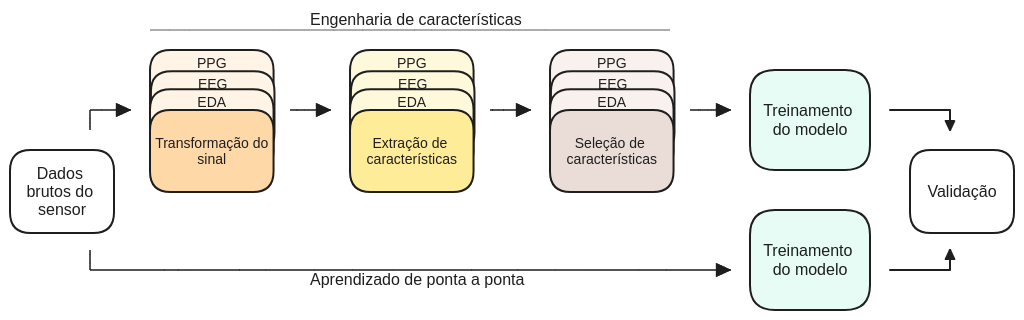
\includegraphics[scale=0.44]{assets/feature_eng-end_to_end.png}
	\label{fig:feature_eng-end_to_end}
 \tiny
 \sourcemedaddy
\end{figure}

\chapter{Materiais e métodos}


\section{Conjunto de dados}






\section{Pré-processamento}

\section{Treinamento}



\subsection{Espaço de busca de hiperparâmetros}

\section{Avaliação}

\section{Considerações do capítulo}

\chapter{Resultados e Discussão}

\section{Análise Exploratória de Dados}

\section{Pré-processamento}
\label{preprocessing}

\section{Otimização de hiperparâmetros}

\section{Discussão}

\section{Contribuições}

\chapter{Considerações finais}




\bibliography{references/export}

% Glossário
 %\chapter*{GLOSSÁRIO}
\addcontentsline{toc}{chapter}{GLOSSARIO}
\begin{itemize}
    \item DF (Dataframe): Um tipo de tabela estruturada para processamento e análise de dados (semelhante ao Excel) e comum em sistemas utilizando o Spark e a biblioteca Pandas
\end{itemize}

% Elemento opcional. Consiste em uma lista de palavras ou expressões técnicas de uso restrito ou de sentido obscuro, utilizadas no texto, acompanhadas das respectivas definições.

% Apêndice
 %\chapter*{APÊNDICE}
\addcontentsline{toc}{chapter}{APÊNDICE}
Elemento opcional. Texto ou documento elaborado pelo autor, que serve de fundamentação, comprovação e ilustração.

% Anexo
 %\chapter*{ANEXO}
\addcontentsline{toc}{chapter}{ANEXO}
Elemento opcional. Texto ou documento não elaborado pelo autor, que serve de fundamentação, comprovação e ilustração.

% Índice
 %\chapter*{ÍNDICE}
\addcontentsline{toc}{chapter}{ÍNDICE}
Elemento opcional. Consiste em uma lista de autor, título ou assunto em ordem alfabética ou sistemática (por classes, numérica ou cronológica) que remete para as informações contidas no texto.


\end{OnehalfSpace}
\end{document}
